%\chapter{Construcción de supercondensadores}
Un supercondensador es construido simplemente haciendo un sándwich electrodo-separador-electrodo. El electrodo es una lámina del material activo, este puede estar depositado en un colector de corriente, o ser una lámina libre. Por otro lado, el separador es una membrana permeable al electrolito, como puede ser una membrana microporosa o papel filtro de celulosa. Como primera aproximación se procede como la secuencia de la figura \ref{fig:SC_process}. 

\begin{figure}[h!]
	\centering
	\fbox{
		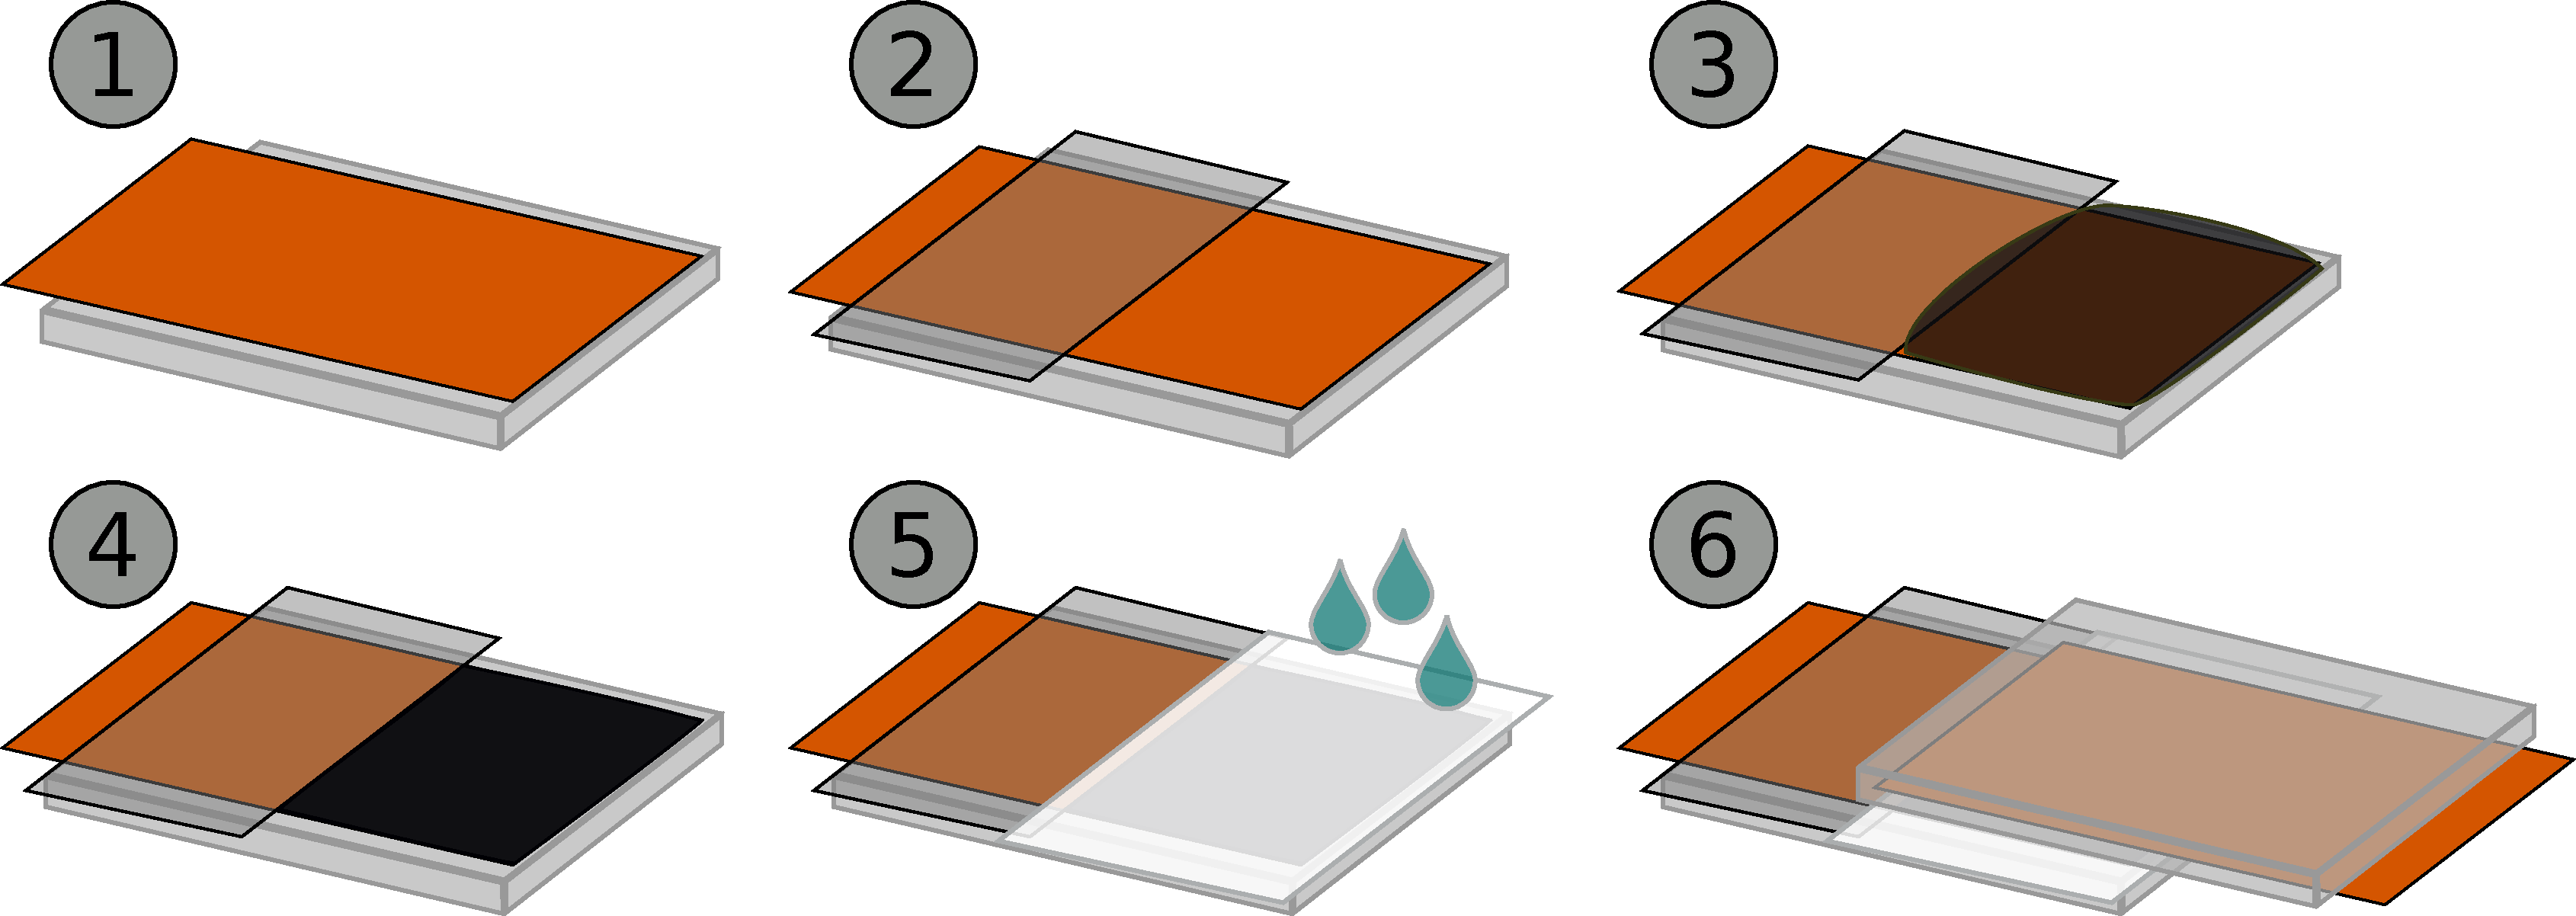
\includegraphics[width = 0.9\textwidth]{SC_process.pdf}
		}
	\caption{}
	\label{fig:SC_process}
\end{figure}

\section{Celda de pruebas de supercondensador}
La construcción de supercondensadores como se detalla anteriormente, presenta varios inconvenientes: (1) la deposición de material en los colectores de corriente no es homogénea, (2) el agua del electrolito se evapora rápidamente, (3) el cierre del dispositivo no es estable, y por consiguiente (4) la conexión a los terminales no es segura. Por estas razones, se diseña una celda que de pruebas que solucione estos problemas.
La celda diseñada y construida (ver figura \ref{fig:celda_de_pruebas_SC}) consta de dos colectores de corriente de acero inoxidable, entre los que se ubica el condensador como tal. Los colectores de corriente tienen sellos que impiden la fuga del electrolito o la evaporación del agua en él, permitiendo una operación estable en el tiempo. Los colectores de corriente se apoyan en bloques de acero que cierran la celda con pernos y permiten conectar los terminales del potenciostato a la celda de pruebas.

\begin{figure}[h!]
	\centering
	\fbox{
		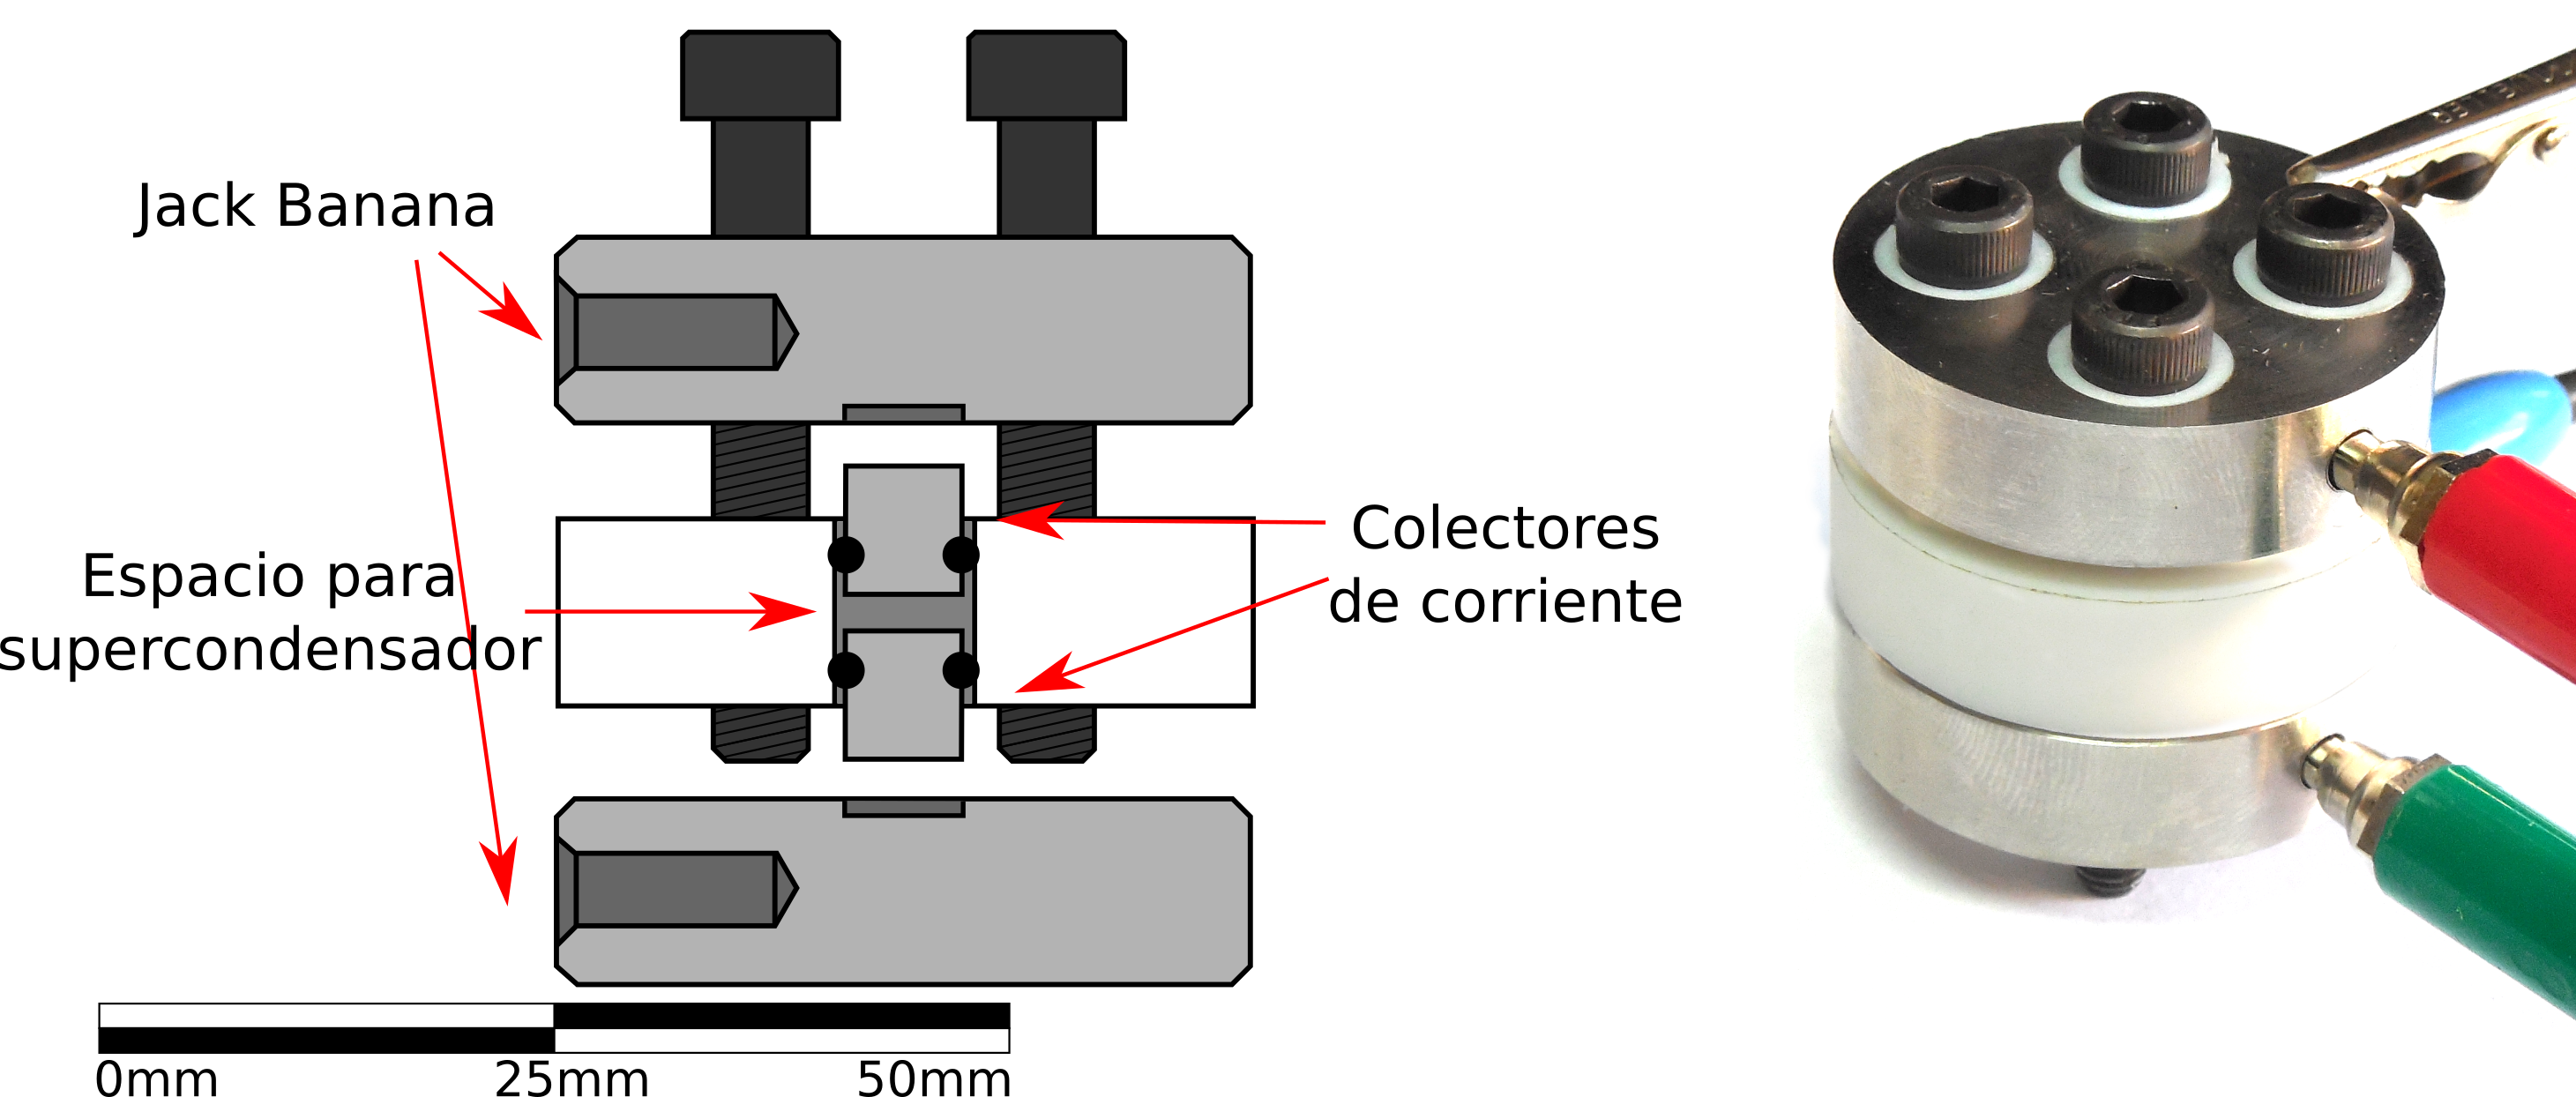
\includegraphics[width=0.8\textwidth]{cell3.pdf}
		}
	\caption[Celda de pruebas de supercondensador.]{Izquierda: Vista longitudinal de la celda de pruebas, mostrando los componentes más importantes. Derecha: Fotografía de la celda armada y conectada al potenciostato.}
	\label{fig:celda_de_pruebas_SC}
\end{figure}

\section{Construcción de electrodos}
Se fabrican seis pares de electrodos utilizando el mismo material sintetizado, pero diferentes sustratos y diferentes métodos de deposisión. Se utilizan dos tipos de sustratos, el primero es un disco de acero 316 de 7 mm de díametro, el segundo es un disco de espuma de níquel también de 7 mm de diámetro. Para fabricar el primer par de electrodos, el material en forma de polvo es dispersado en etilenglicol por medio de ultrasonido, y depositado por goteo en sustrato de acero calentado a 150 \degree C hasta que se recubra el sustrato completamente. Para añadirle PMMA, este se disuelve en acetona a una concentración de 10 mg/ml, solución donde se dispersa el óxido reducido de grafeno por medio de ultrasonido y luego es depositada por goteo en el sustrato de acero a 50 \degree C. De forma análoga, se deposita el material en el sustrato de níquel.
Los electrodos de rGO en forma de papel son fabricados mediante filtración por vacío. En este método, se dispersa el rGO en agua, la que se pasa por un filtro de celulosa en un embudo Büchner conectado a un kitasato y una bomba de vacío, el filtro con el material atrapado se deja secar a temperatura ambiente formando una lámina, la que es desprendida con facilidad del filtro de celulosa y luego recortada al tamaño apropiado para la celda de pruebas. El material dispersado en agua puede ser lyofilizado, obteniendo una espuma de rGO que es utilizada como electrodo en la celda.
La masa del material depositado se mide en una balanza analítica () masando los sustratos antes y después de depositado el material, teniendo la precaución que el solvente se haya evaporado totalmente. Para los electrodos en forma de papel, se masan 20 discos similares y se calcula la masa promedio de cada uno, mientras que el material liofilizado se masa directamente la cantidad a utilizar en la celda de pruebas.

\begin{table}[htbp]
	\centering
	\caption{asd}
	\begin{tabular}{ l l l l }
		Sustrato & Forma & Binder & Masa [mg] \\ \hline
		Acero    & Polvo & -      & 0,4 $\pm$ 0,2 \\
		Acero    & Polvo & PMMA   & 2,8 $\pm$ 0,2 \\
		Acero    & Papel & -      & 0,6 $\pm$ 0,2 \\
		Acero    & Lyo   & -      & 0,6 $\pm$ 0,2 \\
		Nickel   & Polvo & -      & 0,9 $\pm$ 0,2 \\
		Nickel   & Polvo & PMMA   & 0,8 $\pm$ 0,2 \\
	\end{tabular}
	\label{tab:Electrodos construidos}
\end{table}

\pgfplotstabletypeset[
col sep=space,
columns/E/.style={string type}
]{./Data/CV_CRGO300517_11/raw/mass.txt}

\begin{figure}
	\centering
	\fbox{
		\includegraphics[width=1.0\textwidth]{rgo_electrodes.png}
		}
	\caption[Electrodos utilizados en la celda de pruebas de supercondensador.]{Electrodos utilizados en la celda de pruebas de supercondensador. De izquierda a derecha: Electro sin material depositado. Electrodo con material depositado mediante goteo (\emph{drop-casting}). Electrodo con material en forma de papel descentrado. Electrodo con material en forma de papel bien centrado soble el metal.}
	\label{fig:electrodes}
\end{figure}

\section{Resultados}
Los electrodos son sometidos a pruebas electroquímicas para estudiar su desempeño, estás pruebas incluyen: voltametría cíclica (CV), ciclos de carga y descarga a corriente constante, espectroscopía de impedancia electroquímica (EIS). Todas las mediciones electroquímicas son hechas con un potenciostato/galvanostato (Interface 5000E, Gamry). Además de los electrodos construidos con rGO, también se mide el comportamiento de los sustratos sin agregados.

%Resultados
\SCGraphsNoMass{CV_Steel_Disk_No_Material_1}{CV_Steel_Disk_No_Material_2}{0}{16}{1954.91833300000}{Disco de acero sin material.}
\SCGraphs{CV_CRGO300517_9}{CV_CRGO300517_10}{0.0004}{10}{3101.89233300000}{Polvo en disco de acero. Masa = 0.4 mg.}
\SCGraphs{CV_CRGO300517_3}{CV_CRGO300517_4}{0.0028}{20}{2105.33533300000}{Polvo + PMMA en disco de acero. Masa = 2.8 mg.}
\SCGraphs{CV_CRGO300517_11}{CV_CRGO300517_12}{0.0006}{250}{45656.2866670000}{Papel en disco de acero. Masa = 0.6 mg.}
\SCGraphs{CV_CRGO300517_13}{CV_CRGO300517_14}{0.0006}{465}{86333.0367000000}{Material liofilizado en disco de acero. Masa = 0.6 mg.}


\SCGraphsNoMass{CV_Nickel_Foam_No_Material_1}{CV_Nickel_Foam_No_Material_2}{0}{12}{2399.28233300000}{Espuma de níquel sin material.}
\SCGraphs{CV_CRGO300517_5}{CV_CRGO300517_6}{0.0009}{12}{4328.46733300000}{Polvo en espuma de níquel. Masa = 0.9 mg.}
\SCGraphs{CV_CRGO300517_7}{CV_CRGO300517_8}{0.0008}{5}{771.593133000000}{Polvo + PMMA en espuma de níquel. Masa = 0.8 mg.}



%%%%%%%%%%%%%%%%%%%%%%%%%%%%%%%%%%%%%%%%%%%%%%%%%
%%%%%% Paper on steel disk. mass = 0.6 mg %%%%%%%
%%%%%%%%%%%%%%%%%%%%%%%%%%%%%%%%%%%%%%%%%%%%%%%%%
\begin{figure}
	\centering
	\begin{subfigure}{\plotwidth}
		\begin{tikzpicture}[scale=\plotscale,trim axis right,trim axis left]
			\begin{axis}[CVStyle]
				\addplot table [x=Voltaje, y expr=\thisrow{Corriente}/0.0006 ] {./Data/CV_CRGO300517_11/raw/sample1.txt};
				\addplot table [x=Voltaje, y expr=\thisrow{Corriente}/0.0006 ] {./Data/CV_CRGO300517_11/raw/sample2.txt};
				\addplot table [x=Voltaje, y expr=\thisrow{Corriente}/0.0006 ] {./Data/CV_CRGO300517_11/raw/sample3.txt};
				\addplot table [x=Voltaje, y expr=\thisrow{Corriente}/0.0006 ] {./Data/CV_CRGO300517_11/raw/sample4.txt};
				\addplot table [x=Voltaje, y expr=\thisrow{Corriente}/0.0006 ] {./Data/CV_CRGO300517_11/raw/sample5.txt};	
			\end{axis}
		\end{tikzpicture}
	\end{subfigure}\hfill
	\begin{subfigure}{\plotwidth}
		\begin{tikzpicture}[scale=\plotscale,trim axis right,trim axis left]
			\begin{axis}[CVStyle]
				\addplot table [x=Voltaje, y expr=\thisrow{Corriente}/0.0006 ] {./Data/CV_CRGO300517_12/raw/sample1.txt};
				\addplot table [x=Voltaje, y expr=\thisrow{Corriente}/0.0006 ] {./Data/CV_CRGO300517_12/raw/sample2.txt};
				\addplot table [x=Voltaje, y expr=\thisrow{Corriente}/0.0006 ] {./Data/CV_CRGO300517_12/raw/sample3.txt};
				\addplot table [x=Voltaje, y expr=\thisrow{Corriente}/0.0006 ] {./Data/CV_CRGO300517_12/raw/sample4.txt};
				\addplot table [x=Voltaje, y expr=\thisrow{Corriente}/0.0006 ] {./Data/CV_CRGO300517_12/raw/sample5.txt};	
			\end{axis}
		\end{tikzpicture}
	\end{subfigure}\\
	\begin{subfigure}{\plotwidth}
		\begin{tikzpicture}[scale=\plotscale,trim axis right,trim axis left]
			\begin{axis}[CCDStyle]
				\addplot+[restrict x to domain=0:250] table [ x expr=\thisrow{Time}-0, y expr=\thisrow{Voltage} ] {./Data/CV_CRGO300517_11/raw/chargedischarge.txt};	
				\addplot+[restrict x to domain=0:250] table [ x expr=\thisrow{Time}-45656.2866670000, y expr=\thisrow{Voltage} ] {./Data/CV_CRGO300517_11/raw/chargedischarge.txt};
			\end{axis}
		\end{tikzpicture}
	\end{subfigure}\hfill
	\begin{subfigure}{\plotwidth}
		\begin{tikzpicture}[scale=\plotscale,trim axis right,trim axis left]
			\pgfplotstableread{./Data/CV_CRGO300517_11/raw/eisgalv.txt}{\eistable};
			\pgfplotstablegetrowsof{\eistable}
			\pgfmathsetmacro{\N}{\pgfplotsretval}
			\begin{axis}[EISStyle]
			\addplot table [only marks, x=Zreal, y expr=\thisrow{Zimag}*-1] {\eistable}
			node[pos=(1-1)/(\N-1), pin=right:{1 MHz}]{}
			node[pos=(\N-1)/(\N-1), pin=left:{0,1 Hz}]{};
			\end{axis}
		\end{tikzpicture}
	\end{subfigure}\\
	\begin{subfigure}{\plotwidth}
		\begin{tikzpicture}[scale=\plotscale,trim axis right,trim axis left]
			\begin{axis}[SCStyle]
				\addplot table [only marks] {./Data/CV_CRGO300517_11/raw/capacitance.txt};
				\addplot table [only marks] {./Data/CV_CRGO300517_12/raw/capacitance.txt};	
			\end{axis}
		\end{tikzpicture}
	\end{subfigure}\hfill	
	\begin{subfigure}{\plotwidth}
		\begin{tikzpicture}[scale=\plotscale,trim axis right,trim axis left]
			\begin{axis}[CVStyle,
						legend entries={25mV/s antes, 25MV/s después,  400mV/s antes, 400mV/s después}]
				\addplot table [x=Voltaje, y expr=\thisrow{Corriente}/0.0006 ] {./Data/CV_CRGO300517_11/raw/sample1.txt};
				\addplot table [x=Voltaje, y expr=\thisrow{Corriente}/0.0006 ] {./Data/CV_CRGO300517_12/raw/sample1.txt};
				\addplot table [x=Voltaje, y expr=\thisrow{Corriente}/0.0006 ] {./Data/CV_CRGO300517_11/raw/sample5.txt};
				\addplot table [x=Voltaje, y expr=\thisrow{Corriente}/0.0006 ] {./Data/CV_CRGO300517_12/raw/sample5.txt};
			\end{axis}
		\end{tikzpicture}
	\end{subfigure}
	\caption{Paper on steel disk. mass = 0.6 mg}
\end{figure}


%%%%%%%%%%%%%%%%%%%%%%%%%%%%%%%%%%%%%%%%%%%%%%%%
%%%%%% Lyo on steel disk. mass = 0.6 mg %%%%%%%
%%%%%%%%%%%%%%%%%%%%%%%%%%%%%%%%%%%%%%%%%%%%%%%%%
\begin{figure}
	\centering
	\begin{subfigure}{\plotwidth}
		\begin{tikzpicture}[scale=\plotscale,trim axis right,trim axis left]
		\begin{axis}[CVStyle]
		\addplot table [x=Voltaje, y expr=\thisrow{Corriente}/0.0006 ] {./Data/CV_CRGO300517_13/raw/sample1.txt};
		\addplot table [x=Voltaje, y expr=\thisrow{Corriente}/0.0006 ] {./Data/CV_CRGO300517_13/raw/sample2.txt};
		\addplot table [x=Voltaje, y expr=\thisrow{Corriente}/0.0006 ] {./Data/CV_CRGO300517_13/raw/sample3.txt};
		\addplot table [x=Voltaje, y expr=\thisrow{Corriente}/0.0006 ] {./Data/CV_CRGO300517_13/raw/sample4.txt};
		\addplot table [x=Voltaje, y expr=\thisrow{Corriente}/0.0006 ] {./Data/CV_CRGO300517_13/raw/sample5.txt};	
		\end{axis}
		\end{tikzpicture}
	\end{subfigure}\hfill
	\begin{subfigure}{\plotwidth}
		\begin{tikzpicture}[scale=\plotscale,trim axis right,trim axis left]
		\begin{axis}[CVStyle]
		\addplot table [x=Voltaje, y expr=\thisrow{Corriente}/0.0006 ] {./Data/CV_CRGO300517_14/raw/sample1.txt};
		\addplot table [x=Voltaje, y expr=\thisrow{Corriente}/0.0006 ] {./Data/CV_CRGO300517_14/raw/sample2.txt};
		\addplot table [x=Voltaje, y expr=\thisrow{Corriente}/0.0006 ] {./Data/CV_CRGO300517_14/raw/sample3.txt};
		\addplot table [x=Voltaje, y expr=\thisrow{Corriente}/0.0006 ] {./Data/CV_CRGO300517_14/raw/sample4.txt};
		\addplot table [x=Voltaje, y expr=\thisrow{Corriente}/0.0006 ] {./Data/CV_CRGO300517_14/raw/sample5.txt};	
		\end{axis}
		\end{tikzpicture}
	\end{subfigure}\\
	\begin{subfigure}{\plotwidth}
		\begin{tikzpicture}[scale=\plotscale,trim axis right,trim axis left]
		\begin{axis}[CCDStyle]
		\addplot+[restrict x to domain=0:465] table [ x expr=\thisrow{Time}-0, y expr=\thisrow{Voltage} ] {./Data/CV_CRGO300517_13/raw/chargedischarge.txt};	
		\addplot+[restrict x to domain=0:465] table [ x expr=\thisrow{Time}-86333.0367000000, y expr=\thisrow{Voltage} ] {./Data/CV_CRGO300517_13/raw/chargedischarge.txt};
		\end{axis}
		\end{tikzpicture}
	\end{subfigure}\hfill
	\begin{subfigure}{\plotwidth}
		\begin{tikzpicture}[scale=\plotscale,trim axis right,trim axis left]
		\pgfplotstableread{./Data/CV_CRGO300517_13/raw/eisgalv.txt}{\eistable};
		\pgfplotstablegetrowsof{\eistable}
		\pgfmathsetmacro{\N}{\pgfplotsretval}
		\begin{axis}[EISStyle]
		\addplot table [only marks, x=Zreal, y expr=\thisrow{Zimag}*-1] {\eistable}
		node[pos=(1-1)/(\N-1), pin=right:{1 MHz}]{}
		node[pos=(\N-1)/(\N-1), pin=left:{0,1 Hz}]{};
		\end{axis}
		\end{tikzpicture}
	\end{subfigure}\\
	\begin{subfigure}{\plotwidth}
		\begin{tikzpicture}[scale=\plotscale,trim axis right,trim axis left]
		\begin{axis}[SCStyle]
		\addplot table [only marks] {./Data/CV_CRGO300517_13/raw/capacitance.txt};
		\addplot table [only marks] {./Data/CV_CRGO300517_14/raw/capacitance.txt};	
		\end{axis}
		\end{tikzpicture}
	\end{subfigure}\hfill	
	\begin{subfigure}{\plotwidth}
		\begin{tikzpicture}[scale=\plotscale,trim axis right,trim axis left]
		\begin{axis}[CVStyle,
		legend entries={25mV/s antes, 25mV/s después,  400mV/s antes, 400mV/s después}]
		\addplot table [x=Voltaje, y expr=\thisrow{Corriente}/0.0006 ] {./Data/CV_CRGO300517_13/raw/sample1.txt};
		\addplot table [x=Voltaje, y expr=\thisrow{Corriente}/0.0006 ] {./Data/CV_CRGO300517_14/raw/sample1.txt};
		\addplot table [x=Voltaje, y expr=\thisrow{Corriente}/0.0006 ] {./Data/CV_CRGO300517_13/raw/sample5.txt};
		\addplot table [x=Voltaje, y expr=\thisrow{Corriente}/0.0006 ] {./Data/CV_CRGO300517_14/raw/sample5.txt};
		\end{axis}
		\end{tikzpicture}
	\end{subfigure}
	\caption{Lyo on steel disk. mass = 0.6 mg}
\end{figure}



%%%%%%%%%%%%%%%%%%%%%%%%%%%%%%%%%%%%%%%%%%%%%%%%%%
%%% powder + pmma on Steel Disk. mass = 2.8 mg %%%
%%%%%%%%%%%%%%%%%%%%%%%%%%%%%%%%%%%%%%%%%%%%%%%%%%
\begin{figure}
	\centering
	\begin{subfigure}{\plotwidth}
		\begin{tikzpicture}[scale=\plotscale,trim axis right,trim axis left]
			\begin{axis}[CVStyle]
				\addplot table [x=Voltaje, y expr=\thisrow{Corriente}/0.0028 ] {./Data/CV_CRGO300517_3/raw/sample1.txt};
				\addplot table [x=Voltaje, y expr=\thisrow{Corriente}/0.0028 ] {./Data/CV_CRGO300517_3/raw/sample2.txt};
				\addplot table [x=Voltaje, y expr=\thisrow{Corriente}/0.0028 ] {./Data/CV_CRGO300517_3/raw/sample3.txt};
				\addplot table [x=Voltaje, y expr=\thisrow{Corriente}/0.0028 ] {./Data/CV_CRGO300517_3/raw/sample4.txt};
				\addplot table [x=Voltaje, y expr=\thisrow{Corriente}/0.0028 ] {./Data/CV_CRGO300517_3/raw/sample5.txt};	
			\end{axis}
		\end{tikzpicture}
	\end{subfigure}\hfill
	\begin{subfigure}{\plotwidth}
		\begin{tikzpicture}[scale=\plotscale,trim axis right,trim axis left]
			\begin{axis}[CVStyle]
				\addplot[restrict x to domain=-0.8:0.8] table [x=Voltaje, y expr=\thisrow{Corriente}/0.0028 ] {./Data/CV_CRGO300517_4/raw/sample1.txt};
				\addplot table [x=Voltaje, y expr=\thisrow{Corriente}/0.0028 ] {./Data/CV_CRGO300517_4/raw/sample2.txt};
				\addplot table [x=Voltaje, y expr=\thisrow{Corriente}/0.0028 ] {./Data/CV_CRGO300517_4/raw/sample3.txt};
				\addplot table [x=Voltaje, y expr=\thisrow{Corriente}/0.0028 ] {./Data/CV_CRGO300517_4/raw/sample4.txt};
				\addplot table [x=Voltaje, y expr=\thisrow{Corriente}/0.0028 ] {./Data/CV_CRGO300517_4/raw/sample5.txt};	
			\end{axis}
		\end{tikzpicture}
	\end{subfigure}\\
	\begin{subfigure}{\plotwidth}
		\begin{tikzpicture}[scale=\plotscale,trim axis right,trim axis left]
			\begin{axis}[CCDStyle]
				\addplot+[restrict x to domain=0:20] table [x expr=\thisrow{Time}-0, y expr=\thisrow{Voltage}] {./Data/CV_CRGO300517_3/raw/chargedischarge.txt};	
				\addplot+[restrict x to domain=0:20] table [x expr=\thisrow{Time}-2105.33533300000, y expr=\thisrow{Voltage}] {./Data/CV_CRGO300517_3/raw/chargedischarge.txt};
			\end{axis}
		\end{tikzpicture}
	\end{subfigure}\hfill
	\begin{subfigure}{\plotwidth}
		\begin{tikzpicture}[scale=\plotscale,trim axis right,trim axis left]
			\pgfplotstableread{./Data/CV_CRGO300517_3/raw/eisgalv.txt}{\eistable};
			\pgfplotstablegetrowsof{\eistable}
			\pgfmathsetmacro{\N}{\pgfplotsretval}
			\begin{axis}[EISStyle]
			\addplot table [only marks, x=Zreal, y expr=\thisrow{Zimag}*-1] {\eistable}
			node[pos=(1-1)/(\N-1), pin=right:{1 MHz}]{}
			node[pos=(\N-1)/(\N-1), pin=left:{0,1 Hz}]{};
			\end{axis}
		\end{tikzpicture}
	\end{subfigure}\\
	\begin{subfigure}{\plotwidth}
		\begin{tikzpicture}[scale=\plotscale,trim axis right,trim axis left]
			\begin{axis}[SCStyle]
				\addplot table [only marks] {./Data/CV_CRGO300517_3/raw/capacitance.txt};
				\addplot table [only marks] {./Data/CV_CRGO300517_4/raw/capacitance.txt};	
			\end{axis}
		\end{tikzpicture}
	\end{subfigure}\hfill
	\begin{subfigure}{\plotwidth}
		\begin{tikzpicture}[scale=\plotscale,trim axis right,trim axis left]
			\begin{axis}[CVStyle,
			legend entries={25mV/s antes,25MV/s después,  400mV/s antes, 400mV/s después}]
				\addplot table [x=Voltaje, y expr=\thisrow{Corriente}/0.0028 ] {./Data/CV_CRGO300517_3/raw/sample1.txt};
				\addplot table [x=Voltaje, y expr=\thisrow{Corriente}/0.0028 ] {./Data/CV_CRGO300517_4/raw/sample1.txt};
				\addplot table [x=Voltaje, y expr=\thisrow{Corriente}/0.0028 ] {./Data/CV_CRGO300517_3/raw/sample5.txt};
				\addplot table [x=Voltaje, y expr=\thisrow{Corriente}/0.0028 ] {./Data/CV_CRGO300517_4/raw/sample5.txt};
			\end{axis}
		\end{tikzpicture}
	\end{subfigure}
	\caption{powder + pmma on Steel Disk. mass = 2.8 mg}
\end{figure}

%%%%%%%%%%%%%%%%%%%%%%%%%%%%%%%%%%%%%%%
%%%%% powder on Ni Foam m = 0.9 mg %%%%
%%%%%%%%%%%%%%%%%%%%%%%%%%%%%%%%%%%%%%%
\begin{figure}
	\centering
	\begin{subfigure}{\plotwidth}
		\begin{tikzpicture}[scale=\plotscale,trim axis right,trim axis left]
			\begin{axis}[CVStyle]
				\addplot table [x=Voltaje, y expr=\thisrow{Corriente}/0.0009 ] {./Data/CV_CRGO300517_5/raw/sample1.txt};
				\addplot table [x=Voltaje, y expr=\thisrow{Corriente}/0.0009 ] {./Data/CV_CRGO300517_5/raw/sample2.txt};
				\addplot table [x=Voltaje, y expr=\thisrow{Corriente}/0.0009 ] {./Data/CV_CRGO300517_5/raw/sample3.txt};
				\addplot table [x=Voltaje, y expr=\thisrow{Corriente}/0.0009 ] {./Data/CV_CRGO300517_5/raw/sample4.txt};
				\addplot table [x=Voltaje, y expr=\thisrow{Corriente}/0.0009 ] {./Data/CV_CRGO300517_5/raw/sample5.txt};	
			\end{axis}
		\end{tikzpicture}
	\end{subfigure}\hfill
	\begin{subfigure}{\plotwidth}
		\begin{tikzpicture}[scale=\plotscale,trim axis right,trim axis left]
			\begin{axis}[CVStyle]
				\addplot table [x=Voltaje, y expr=\thisrow{Corriente}/0.0009 ] {./Data/CV_CRGO300517_6/raw/sample1.txt};
				\addplot table [x=Voltaje, y expr=\thisrow{Corriente}/0.0009 ] {./Data/CV_CRGO300517_6/raw/sample2.txt};
				\addplot table [x=Voltaje, y expr=\thisrow{Corriente}/0.0009 ] {./Data/CV_CRGO300517_6/raw/sample3.txt};
				\addplot table [x=Voltaje, y expr=\thisrow{Corriente}/0.0009 ] {./Data/CV_CRGO300517_6/raw/sample4.txt};
				\addplot table [x=Voltaje, y expr=\thisrow{Corriente}/0.0009 ] {./Data/CV_CRGO300517_6/raw/sample5.txt};	
			\end{axis}
		\end{tikzpicture}
	\end{subfigure}\\
	\begin{subfigure}{\plotwidth}
		\begin{tikzpicture}[scale=\plotscale,trim axis right,trim axis left]
			\begin{axis}[CCDStyle]
				\addplot+[restrict x to domain=0:12] table [x expr=\thisrow{Time}-0, y expr=\thisrow{Voltage}] {./Data/CV_CRGO300517_5/raw/chargedischarge.txt};	
				\addplot+[restrict x to domain=0:12] table [x expr=\thisrow{Time}-4328.46733300000, y expr=\thisrow{Voltage}] {./Data/CV_CRGO300517_5/raw/chargedischarge.txt};
			\end{axis}
		\end{tikzpicture}
	\end{subfigure}\hfill
	\begin{subfigure}{\plotwidth}
		\begin{tikzpicture}[scale=\plotscale,trim axis right,trim axis left]
			\pgfplotstableread{./Data/CV_CRGO300517_5/raw/eisgalv.txt}{\eistable};
			\pgfplotstablegetrowsof{\eistable}
			\pgfmathsetmacro{\N}{\pgfplotsretval}
			\begin{axis}[EISStyle]
			\addplot table [only marks, x=Zreal, y expr=\thisrow{Zimag}*-1] {\eistable}
			node[pos=(1-1)/(\N-1), pin=right:{1 MHz}]{}
			node[pos=(\N-1)/(\N-1), pin=below:{0,1 Hz}]{};
			\end{axis}
		\end{tikzpicture}
	\end{subfigure}\\
	\begin{subfigure}{\plotwidth}
		\begin{tikzpicture}[scale=\plotscale,trim axis right,trim axis left]
		\begin{axis}[SCStyle]
		\addplot table [only marks] {./Data/CV_CRGO300517_5/raw/capacitance.txt};
		\addplot table [only marks] {./Data/CV_CRGO300517_6/raw/capacitance.txt};	
		\end{axis}
		\end{tikzpicture}
	\end{subfigure}\hfill
	\begin{subfigure}{\plotwidth}
		\begin{tikzpicture}[scale=\plotscale,trim axis right,trim axis left]
			\begin{axis}[CVStyle,
			legend entries={25mV/s antes,25MV/s después,  400mV/s antes, 400mV/s después}]
				\addplot table [x=Voltaje, y expr=\thisrow{Corriente}/0.0009 ] {./Data/CV_CRGO300517_5/raw/sample1.txt};
				\addplot table [x=Voltaje, y expr=\thisrow{Corriente}/0.0009 ] {./Data/CV_CRGO300517_6/raw/sample1.txt};
				\addplot table [x=Voltaje, y expr=\thisrow{Corriente}/0.0009 ] {./Data/CV_CRGO300517_5/raw/sample5.txt};
				\addplot table [x=Voltaje, y expr=\thisrow{Corriente}/0.0009 ] {./Data/CV_CRGO300517_6/raw/sample5.txt};
			\end{axis}
		\end{tikzpicture}
	\end{subfigure}
	\caption{powder on Ni Foam m = 0.9 mg}
\end{figure}

%%%%%%%%%%%%%%%%%%%%%%%%%%%%%%%%%%%%%%%
%%%%% powder + pmma on Ni Foam m = 0.8 mg %%%%
%%%%%%%%%%%%%%%%%%%%%%%%%%%%%%%%%%%%%%%
\begin{figure}
	\centering
	\begin{subfigure}{\plotwidth}
		\begin{tikzpicture}[scale=\plotscale,trim axis right,trim axis left]
		\begin{axis}[CVStyle]
		\addplot table [x=Voltaje, y expr=\thisrow{Corriente}/0.0008 ] {./Data/CV_CRGO300517_7/raw/sample1.txt};
		\addplot table [x=Voltaje, y expr=\thisrow{Corriente}/0.0008 ] {./Data/CV_CRGO300517_7/raw/sample2.txt};
		\addplot table [x=Voltaje, y expr=\thisrow{Corriente}/0.0008 ] {./Data/CV_CRGO300517_7/raw/sample3.txt};
		\addplot table [x=Voltaje, y expr=\thisrow{Corriente}/0.0008 ] {./Data/CV_CRGO300517_7/raw/sample4.txt};
		\addplot table [x=Voltaje, y expr=\thisrow{Corriente}/0.0008 ] {./Data/CV_CRGO300517_7/raw/sample5.txt};	
		\end{axis}
		\end{tikzpicture}
	\end{subfigure}\hfill
	\begin{subfigure}{\plotwidth}
		\begin{tikzpicture}[scale=\plotscale,trim axis right,trim axis left]
			\begin{axis}[CVStyle]
				\addplot table [x=Voltaje, y expr=\thisrow{Corriente}/0.0008 ] {./Data/CV_CRGO300517_8/raw/sample1.txt};
				\addplot table [x=Voltaje, y expr=\thisrow{Corriente}/0.0008 ] {./Data/CV_CRGO300517_8/raw/sample2.txt};
				\addplot table [x=Voltaje, y expr=\thisrow{Corriente}/0.0008 ] {./Data/CV_CRGO300517_8/raw/sample3.txt};
				\addplot table [x=Voltaje, y expr=\thisrow{Corriente}/0.0008 ] {./Data/CV_CRGO300517_8/raw/sample4.txt};
				\addplot table [x=Voltaje, y expr=\thisrow{Corriente}/0.0008 ] {./Data/CV_CRGO300517_8/raw/sample5.txt};	
			\end{axis}
		\end{tikzpicture}
	\end{subfigure}\\
	\begin{subfigure}{\plotwidth}
		\begin{tikzpicture}[scale=\plotscale,trim axis right,trim axis left]
			\begin{axis}[CCDStyle]
				\addplot+[restrict x to domain=0:5] table [x expr=\thisrow{Time}-0, y expr=\thisrow{Voltage}] {./Data/CV_CRGO300517_7/raw/chargedischarge.txt};	
				\addplot+[restrict x to domain=0:5] table [x expr=\thisrow{Time}-771.593133000000, y expr=\thisrow{Voltage}] {./Data/CV_CRGO300517_7/raw/chargedischarge.txt};
			\end{axis}
		\end{tikzpicture}
	\end{subfigure}\hfill
	\begin{subfigure}{\plotwidth}
		\begin{tikzpicture}[scale=\plotscale,trim axis right,trim axis left]
			\pgfplotstableread{./Data/CV_CRGO300517_7/raw/eisgalv.txt}{\eistable};
			\pgfplotstablegetrowsof{\eistable}
			\pgfmathsetmacro{\N}{\pgfplotsretval}
			\begin{axis}[EISStyle]
			\addplot table [only marks, x=Zreal, y expr=\thisrow{Zimag}*-1] {\eistable}
			node[pos=(1-1)/(\N-1), pin=right:{1 MHz}]{}
			node[pos=(\N-1)/(\N-1), pin=left:{0,1 Hz}]{};
			\end{axis}
		\end{tikzpicture}
	\end{subfigure}\\
	\begin{subfigure}{\plotwidth}
		\begin{tikzpicture}[scale=\plotscale,trim axis right,trim axis left]
			\begin{axis}[SCStyle]
				\addplot table [only marks] {./Data/CV_CRGO300517_7/raw/capacitance.txt};	
				\addplot table [only marks] {./Data/CV_CRGO300517_8/raw/capacitance.txt};	
			\end{axis}
		\end{tikzpicture}
	\end{subfigure}\hfill
	\begin{subfigure}{\plotwidth}
		\begin{tikzpicture}[scale=\plotscale,trim axis right,trim axis left]
			\begin{axis}[CVStyle,
			legend entries={25mV/s antes,25MV/s después,  400mV/s antes, 400mV/s después}]
				\addplot table [x=Voltaje, y expr=\thisrow{Corriente}/0.0008 ] {./Data/CV_CRGO300517_7/raw/sample1.txt};
				\addplot table [x=Voltaje, y expr=\thisrow{Corriente}/0.0008 ] {./Data/CV_CRGO300517_8/raw/sample1.txt};
				\addplot table [x=Voltaje, y expr=\thisrow{Corriente}/0.0008 ] {./Data/CV_CRGO300517_7/raw/sample5.txt};
				\addplot table [x=Voltaje, y expr=\thisrow{Corriente}/0.0008 ] {./Data/CV_CRGO300517_8/raw/sample5.txt};
			\end{axis}
		\end{tikzpicture}
	\end{subfigure}
	\caption{powder + pmma on Ni Foam m = 0.8 mg}
\end{figure}

%%%%%%%%%%%%%%%%%%%%%%%%%%%%%%%%%%%%%%%%%%
%%%%% powder on steel disk m = 0.4 mg %%%%
%%%%%%%%%%%%%%%%%%%%%%%%%%%%%%%%%%%%%%%%%%
\begin{figure}
	\centering
	\begin{subfigure}{\plotwidth}
		\begin{tikzpicture}[scale=\plotscale,trim axis right,trim axis left]
			\begin{axis}[CVStyle]
				\addplot table [x=Voltaje, y expr=\thisrow{Corriente}/0.0004 ] {./Data/CV_CRGO300517_9/raw/sample1.txt};
				\addplot table [x=Voltaje, y expr=\thisrow{Corriente}/0.0004 ] {./Data/CV_CRGO300517_9/raw/sample2.txt};
				\addplot table [x=Voltaje, y expr=\thisrow{Corriente}/0.0004 ] {./Data/CV_CRGO300517_9/raw/sample3.txt};
				\addplot table [x=Voltaje, y expr=\thisrow{Corriente}/0.0004 ] {./Data/CV_CRGO300517_9/raw/sample4.txt};
				\addplot table [x=Voltaje, y expr=\thisrow{Corriente}/0.0004 ] {./Data/CV_CRGO300517_9/raw/sample5.txt};	
			\end{axis}
		\end{tikzpicture}
	\end{subfigure}\hfill
	\begin{subfigure}{\plotwidth}
		\begin{tikzpicture}[scale=\plotscale,trim axis right,trim axis left]
			\begin{axis}[CVStyle]
				\addplot table [x=Voltaje, y expr=\thisrow{Corriente}/0.0004 ] {./Data/CV_CRGO300517_10/raw/sample1.txt};
				\addplot table [x=Voltaje, y expr=\thisrow{Corriente}/0.0004 ] {./Data/CV_CRGO300517_10/raw/sample2.txt};
				\addplot table [x=Voltaje, y expr=\thisrow{Corriente}/0.0004 ] {./Data/CV_CRGO300517_10/raw/sample3.txt};
				\addplot table [x=Voltaje, y expr=\thisrow{Corriente}/0.0004 ] {./Data/CV_CRGO300517_10/raw/sample4.txt};
				\addplot table [x=Voltaje, y expr=\thisrow{Corriente}/0.0004 ] {./Data/CV_CRGO300517_10/raw/sample5.txt};	
			\end{axis}
		\end{tikzpicture}
	\end{subfigure}\\
	\begin{subfigure}{\plotwidth}
		\begin{tikzpicture}[scale=\plotscale,trim axis right,trim axis left]
			\begin{axis}[CCDStyle]
				\addplot+[restrict x to domain=0:10] table [x expr=\thisrow{Time}-0, y expr=\thisrow{Voltage}] {./Data/CV_CRGO300517_9/raw/chargedischarge.txt};	
				\addplot+[restrict x to domain=0:10] table [x expr=\thisrow{Time}-3101.89233300000, y expr=\thisrow{Voltage}] {./Data/CV_CRGO300517_9/raw/chargedischarge.txt};
			\end{axis}
		\end{tikzpicture}
	\end{subfigure}\hfill
	\begin{subfigure}{\plotwidth}
		\begin{tikzpicture}[scale=\plotscale,trim axis right,trim axis left]
			\pgfplotstableread{./Data/CV_CRGO300517_9/raw/eisgalv.txt}{\eistable};
			\pgfplotstablegetrowsof{\eistable}
			\pgfmathsetmacro{\N}{\pgfplotsretval}
			\begin{axis}[EISStyle]
			\addplot table [only marks, x=Zreal, y expr=\thisrow{Zimag}*-1] {\eistable}
			node[pos=(1-1)/(\N-1), pin=right:{1 MHz}]{}
			node[pos=(\N-1)/(\N-1), pin=left:{0,1 Hz}]{};
			\end{axis}
		\end{tikzpicture}
	\end{subfigure}\\
	\begin{subfigure}{\plotwidth}
		\begin{tikzpicture}[scale=\plotscale,trim axis right,trim axis left]
			\begin{axis}[SCStyle]
				\addplot table [only marks] {./Data/CV_CRGO300517_9/raw/capacitance.txt};
				\addplot table [only marks] {./Data/CV_CRGO300517_10/raw/capacitance.txt};		
			\end{axis}
		\end{tikzpicture}
	\end{subfigure}\hfill
	\begin{subfigure}{\plotwidth}
		\begin{tikzpicture}[scale=\plotscale,trim axis right,trim axis left]
			\begin{axis}[CVStyle,
			legend entries={25mV/s antes,25MV/s después,  400mV/s antes, 400mV/s después}]
				\addplot table [x=Voltaje, y expr=\thisrow{Corriente}/0.0004 ] {./Data/CV_CRGO300517_9/raw/sample1.txt};
				\addplot table [x=Voltaje, y expr=\thisrow{Corriente}/0.0004 ] {./Data/CV_CRGO300517_10/raw/sample1.txt};
				\addplot table [x=Voltaje, y expr=\thisrow{Corriente}/0.0004 ] {./Data/CV_CRGO300517_9/raw/sample5.txt};
				\addplot table [x=Voltaje, y expr=\thisrow{Corriente}/0.0004 ] {./Data/CV_CRGO300517_10/raw/sample5.txt};
			\end{axis}
		\end{tikzpicture}
	\end{subfigure}
	\caption{powder on steel disk, m = 0,4mg}
\end{figure}

%%%%%%%%%%%%%%%%%%%%%%%%%%%%%%%%%%
%%%%% steel disk, no material %%%%
%%%%%%%%%%%%%%%%%%%%%%%%%%%%%%%%%%
\begin{figure}
	\centering
	\begin{subfigure}{\plotwidth}
		\begin{tikzpicture}[scale=\plotscale,trim axis right,trim axis left]
			\begin{axis}[CVStyle,
			scaled ticks=base 10:3,
			ylabel = {Corriente [A]},]
				\addplot table [x=Voltaje, y expr=\thisrow{Corriente} ] {./Data/CV_Steel_Disk_No_Material_1/raw/sample1.txt};
				\addplot table [x=Voltaje, y expr=\thisrow{Corriente} ] {./Data/CV_Steel_Disk_No_Material_1/raw/sample2.txt};
				\addplot table [x=Voltaje, y expr=\thisrow{Corriente} ] {./Data/CV_Steel_Disk_No_Material_1/raw/sample3.txt};
				\addplot table [x=Voltaje, y expr=\thisrow{Corriente} ] {./Data/CV_Steel_Disk_No_Material_1/raw/sample4.txt};
				\addplot table [x=Voltaje, y expr=\thisrow{Corriente} ] {./Data/CV_Steel_Disk_No_Material_1/raw/sample5.txt};	
			\end{axis}
		\end{tikzpicture}
		\caption{asd}
	\end{subfigure}\hfill
	\begin{subfigure}{\plotwidth}
		\begin{tikzpicture}[scale=\plotscale,trim axis right,trim axis left]
			\begin{axis}[CVStyle,
			scaled ticks=base 10:6,
			ylabel = {Corriente [A]},]
				\addplot table [x=Voltaje, y expr=\thisrow{Corriente} ] {./Data/CV_Steel_Disk_No_Material_2/raw/sample1.txt};
				\addplot table [x=Voltaje, y expr=\thisrow{Corriente} ] {./Data/CV_Steel_Disk_No_Material_2/raw/sample2.txt};
				\addplot table [x=Voltaje, y expr=\thisrow{Corriente} ] {./Data/CV_Steel_Disk_No_Material_2/raw/sample3.txt};
				\addplot table [x=Voltaje, y expr=\thisrow{Corriente} ] {./Data/CV_Steel_Disk_No_Material_2/raw/sample4.txt};
				\addplot table [x=Voltaje, y expr=\thisrow{Corriente} ] {./Data/CV_Steel_Disk_No_Material_2/raw/sample5.txt};	
			\end{axis}
		\end{tikzpicture}
		\caption{asd}
	\end{subfigure}\\
	\begin{subfigure}{\plotwidth}
		\begin{tikzpicture}[scale=\plotscale,trim axis right,trim axis left]
			\begin{axis}[CCDStyle]
				\addplot+[restrict x to domain=0:6] table [x expr=\thisrow{Time}-0, y expr=\thisrow{Voltage}] {./Data/CV_Steel_Disk_No_Material_1/raw/chargedischarge.txt};	
				\addplot+[restrict x to domain=0:6] table [x expr=\thisrow{Time}-1954.91833300000, y expr=\thisrow{Voltage}] {./Data/CV_Steel_Disk_No_Material_1/raw/chargedischarge.txt};
			\end{axis}
		\end{tikzpicture}
		\caption{asd}
	\end{subfigure}\hfill
	\begin{subfigure}{\plotwidth}
		\begin{tikzpicture}[scale=\plotscale,trim axis right,trim axis left]
			\pgfplotstableread{./Data/CV_Steel_Disk_No_Material_1/raw/eisgalv.txt}{\eistable};
			\pgfplotstablegetrowsof{\eistable}
			\pgfmathsetmacro{\N}{\pgfplotsretval}
			\begin{axis}[EISStyle]
			\addplot table [only marks, x=Zreal, y expr=\thisrow{Zimag}*-1] {\eistable}
			node[pos=(1-1)/(\N-1), pin=right:{1 MHz}]{}
			node[pos=(\N-1)/(\N-1), pin=below:{0,1 Hz}]{};
			\end{axis}
		\end{tikzpicture}
		\caption{asd}
	\end{subfigure}\\
	\begin{subfigure}{\plotwidth}
		\begin{tikzpicture}[scale=\plotscale,trim axis right,trim axis left]
		\begin{axis}[SCStyle]
		\addplot table [only marks] {./Data/CV_Steel_Disk_No_Material_1/raw/capacitance.txt};
		\addplot table [only marks] {./Data/CV_Steel_Disk_No_Material_2/raw/capacitance.txt};	
		\end{axis}
		\end{tikzpicture}
		\caption{asd}
	\end{subfigure}\hfill
	\begin{subfigure}{\plotwidth}
		\begin{tikzpicture}[scale=\plotscale,trim axis right,trim axis left]
			\begin{axis}[CVStyle,
			scaled ticks=base 10:6,
			ylabel = {Corriente [A]},
			legend entries={25mV/s antes,25MV/s después,  400mV/s antes, 400mV/s después}]
				\addplot table [x=Voltaje, y expr=\thisrow{Corriente}] {./Data/CV_Steel_Disk_No_Material_1/raw/sample1.txt};
				\addplot table [x=Voltaje, y expr=\thisrow{Corriente}] {./Data/CV_Steel_Disk_No_Material_2/raw/sample1.txt};
				\addplot table [x=Voltaje, y expr=\thisrow{Corriente}] {./Data/CV_Steel_Disk_No_Material_1/raw/sample5.txt};
				\addplot table [x=Voltaje, y expr=\thisrow{Corriente}] {./Data/CV_Steel_Disk_No_Material_2/raw/sample5.txt};
			\end{axis}
		\end{tikzpicture}
		\caption{asd}
	\end{subfigure}
	
	\caption{Steel disk no material.}
\end{figure}


%%%%%%%%%%%%%%%%%%%%%%%%%%%%%%%%%%%
%%%%% Nickel Foam, no material %%%%
%%%%%%%%%%%%%%%%%%%%%%%%%%%%%%%%%%%
\begin{figure}
	\centering
	\begin{subfigure}{\plotwidth}
		\begin{tikzpicture}[scale=\plotscale,trim axis right,trim axis left]
			\begin{axis}[CVStyle,
			scaled ticks=base 10:6,
			ylabel = {Corriente [A]},]
				\addplot table [x=Voltaje, y expr=\thisrow{Corriente} ] {./Data/CV_Nickel_Foam_No_Material_1/raw/sample1.txt};
				\addplot table [x=Voltaje, y expr=\thisrow{Corriente} ] {./Data/CV_Nickel_Foam_No_Material_1/raw/sample2.txt};
				\addplot table [x=Voltaje, y expr=\thisrow{Corriente} ] {./Data/CV_Nickel_Foam_No_Material_1/raw/sample3.txt};
				\addplot table [x=Voltaje, y expr=\thisrow{Corriente} ] {./Data/CV_Nickel_Foam_No_Material_1/raw/sample4.txt};
				\addplot table [x=Voltaje, y expr=\thisrow{Corriente} ] {./Data/CV_Nickel_Foam_No_Material_1/raw/sample5.txt};	
			\end{axis}
		\end{tikzpicture}
	\end{subfigure}\hfill
	\begin{subfigure}{\plotwidth}
		\begin{tikzpicture}[scale=\plotscale,trim axis right,trim axis left]
			\begin{axis}[CVStyle,
			scaled ticks=base 10:6,
			ylabel = {Corriente [A]},]
				\addplot table [x=Voltaje, y expr=\thisrow{Corriente} ] {./Data/CV_Nickel_Foam_No_Material_2/raw/sample1.txt};
				\addplot table [x=Voltaje, y expr=\thisrow{Corriente} ] {./Data/CV_Nickel_Foam_No_Material_2/raw/sample2.txt};
				\addplot table [x=Voltaje, y expr=\thisrow{Corriente} ] {./Data/CV_Nickel_Foam_No_Material_2/raw/sample3.txt};
				\addplot table [x=Voltaje, y expr=\thisrow{Corriente} ] {./Data/CV_Nickel_Foam_No_Material_2/raw/sample4.txt};
				\addplot table [x=Voltaje, y expr=\thisrow{Corriente} ] {./Data/CV_Nickel_Foam_No_Material_2/raw/sample5.txt};	
			\end{axis}
		\end{tikzpicture}
	\end{subfigure}\\
	\begin{subfigure}{\plotwidth}
		\begin{tikzpicture}[scale=\plotscale,trim axis right,trim axis left]
			\begin{axis}[CCDStyle]
				\addplot+[restrict x to domain=0:12] table [x expr=\thisrow{Time}-0, y expr=\thisrow{Voltage}] {./Data/CV_Nickel_Foam_No_Material_1/raw/chargedischarge.txt};	
				\addplot+[restrict x to domain=0:12] table [x expr=\thisrow{Time}-2399.28233300000, y expr=\thisrow{Voltage}] {./Data/CV_Nickel_Foam_No_Material_1/raw/chargedischarge.txt};
			\end{axis}
		\end{tikzpicture}
	\end{subfigure}\hfill
	\begin{subfigure}{\plotwidth}
		\begin{tikzpicture}[scale=\plotscale,trim axis right,trim axis left]
			\pgfplotstableread{./Data/CV_Nickel_Foam_No_Material_1/raw/eisgalv.txt}{\eistable};
			\pgfplotstablegetrowsof{\eistable}
			\pgfmathsetmacro{\N}{\pgfplotsretval}
			\begin{axis}[EISStyle]
			\addplot table [only marks, x=Zreal, y expr=\thisrow{Zimag}*-1] {\eistable}
			node[pos=(1-1)/(\N-1), pin=right:{1 MHz}]{}
			node[pos=(\N-1)/(\N-1), pin=below:{0,1 Hz}]{};
			\end{axis}
		\end{tikzpicture}
	\end{subfigure}\\
	\begin{subfigure}{\plotwidth}
		\begin{tikzpicture}[scale=\plotscale,trim axis right,trim axis left]
			\begin{axis}[SCStyle]
				\addplot table [only marks] {./Data/CV_Nickel_Foam_No_Material_1/raw/capacitance.txt};
				\addplot table [only marks] {./Data/CV_Nickel_Foam_No_Material_2/raw/capacitance.txt};
			\end{axis}
		\end{tikzpicture}
	\end{subfigure}\hfill
	\begin{subfigure}{\plotwidth}
		\begin{tikzpicture}[scale=\plotscale,trim axis right,trim axis left]
			\begin{axis}[CVStyle,
			scaled ticks=base 10:6,
			ylabel = {Corriente [A]},
			legend entries={25mV/s antes,25MV/s después,  400mV/s antes, 400mV/s después}]
				\addplot table [x=Voltaje, y expr=\thisrow{Corriente}] {./Data/CV_Nickel_Foam_No_Material_1/raw/sample1.txt};
				\addplot table [x=Voltaje, y expr=\thisrow{Corriente}] {./Data/CV_Nickel_Foam_No_Material_2/raw/sample1.txt};
				\addplot table [x=Voltaje, y expr=\thisrow{Corriente}] {./Data/CV_Nickel_Foam_No_Material_1/raw/sample5.txt};
				\addplot table [x=Voltaje, y expr=\thisrow{Corriente}] {./Data/CV_Nickel_Foam_No_Material_2/raw/sample5.txt};
			\end{axis}
		\end{tikzpicture}
	\end{subfigure}

	\caption{Nickel Foam no material.}
\end{figure}






